\documentclass{elsart}
\usepackage{amsfonts,epsfig,cite}
\usepackage{graphicx}
\journal{CGTA}

\newtheorem{theorem}{Theorem}
\newtheorem{lemma}{Lemma}
\newtheorem{thma}{Subdivision Lemma}
\newenvironment{proof}{{\bf Proof:} \rm}{\hfill $\Box$ \medskip\\}

\newcommand{\comment}[1]{}
\newcommand{\depth}{\mathrm{depth}}


\comment{
\author{Harish Gopala and Pat Morin%
	\thanks{School of Computer Science,
		Carleton University, 
		1125 Colonel By Drive, 
		Ottawa, CANADA K1S 5B6.
   		\email{\{hgopala,morin\}@scs.carleton.ca}
	}
}
}

\date{}
\begin{document}
\begin{frontmatter}
\title{Algorithms for bivariate zonoid depth}
\author{Harish Gopala and Pat Morin}
\address{School of Computer Science, Carleton University \\
	1125 Colonel By Drive, Ottawa, CANADA K1S~5B6}

\thanks[funding]{This research was partly funded by a grant from the
Natural Sciences and Engineering Research Council of Canada and by an
Ontario Graduate Scholarship.}

\begin{abstract}
Zonoid depth is a definition of data depth proposed by Dyckerhoff et
al.\ \cite{zonoid_data_depth_theory_and_computation}. 
Efficient algorithms for solving several computational problems
related to zonoid depth
in 2-dimensional (bivariate) data sets are studied. These include algorithms
for computing a zonoid depth map, computing a zonoid depth contour,
and computing the zonoid depth of a point.
\end{abstract}
\end{frontmatter}

\section{Introduction}\label{section_introduction}

Data depth is a way of measuring how deep or central a given point $x$
in $\mathbb{R}^d$ is with respect to a given data cloud $\{x_1, x_2,
\ldots, x_n\}$. This concept provides a center-outward ordering of
points in Euclidean space of any dimension and leads to a new
non-parametric multivariate statistical analysis in which no
distribution assumptions are needed. Liu et al.\
\cite{multivariate_analysis_by_data_depth} describe many different
notions of depth such as the half space, the convex hull peeling, the
Oja, the simplicial, the majority, and the likelihood depths. However,
many computational problems associated with such data depth functions
are non-trivial to solve efficiently.  Thus the study of these
functions and related algorithms is essential for these functions to
become more useful in statistics. Computational geometry
\cite{preparata_book} has been of great help in this regard, and there
are many results in the computational geometry literature giving
efficient algorithms for data depth problems
\cite{regression_depth_and_center_points, aloupis_mcs_thesis,
algorithms_for_bivariate_medians_and_a_fermat_torricelli_problem_for_lines,
an_optimized_randomized_algorithm_for_maximum_tukey_depth,
on_khulls_and_related_problems,
zonoid_data_depth_theory_and_computation,
%algorithms_for_bivariate_zonoid_depth,
computing_the_centerpoint_of_a_finite_planar_set_of_points_in_linear_time,
on_a_triangle_counting_problem, langerman_phd_thesis,
the_complexity_of_hyperplane_depth_in_the_plane,
optimization_in_arrangements,
computing_the_center_of_planar_point_sets,
fast_implementation_of_depth_contours_using_topological_sweep,
statistical_algorithms_the_oja_bivariate_median,
efficient_algorithms_for_maximum_regression_depth,
a_lower_bound_for_computing_oja_depth,
on_the_computation_of_the_bivariate_median_and_a_fermat_torricelli_problem,
on_the_convex_layers_of_a_planar_set,
on_algorithms_for_simplicial_depth,
constructing_the_bivariate_tukey_median,
geometry_and_statistics_problems_at_the_interface,
some_new_algorithms_and_software_implementation_methods_for_pattern_recognition_research}.

Here, we focus on one particular depth measure, \emph{zonoid depth},
introduced by Dyckerhoff et al.\
\cite{zonoid_data_depth_theory_and_computation} and which is the topic
of a book by Mosler \cite{mosler_book}.

\subsection{Definition of zonoid depth and regions}
\label{subsection_definition_of_zonoid_depth_and_regions}

Given a set of points $S = \{p_1, p_2,\ldots, p_n\}$ in
$\mathbb{R}^d$, the convex hull of points in $S$ is defined as 
\[
   CH(S) = \left\{\sum_{i=1}^{n} \lambda_ip_i \mid 0 \le \lambda_i \le 1,
             \sum_{i=1}^{n}{\lambda_i} = 1\right\} \enspace . 
\] 
The \emph{$k$-zonoid} (the zonoid of depth $k$) is defined as
\[
   Z_k(S) = \left\{\sum_{i=1}^{n}\lambda_ip_i \mid 0 \le \lambda_i \le
             \frac{1}{k}, \sum_{i=1}^{n}{\lambda_i} = 1\right\}
\] 
Here, and throughout this article, $1 \le k \le n$ is an
integer\footnote{In the zonoid depth literature, the value $k$ may be
any real number between $1$ and $n$. Although the algorithms in this
paper are stated for $k$ being an integer, they extend easily to the
case of real-valued $k$.} and we focus on the special case $d=2$. The
\emph{zonoid depth} of a point $p$ with respect to a set $S$ is
defined as the maximum value $k$ for which $p$ is contained in
$Z_k(S)$.  

Since a zonoid is defined by a finite set of linear constraints, it
forms a convex polygon.  Furthermore, for $k_1 > k_2$, the
$k_1$-zonoid is a subset of the $k_2$-zonoid, hence
$Z_1(S),\ldots,Z_n(S)$ form a sequence of nested convex polygons.  The
$n$-zonoid $Z_n(S)$ contains a single point, the mean of $S$. For other
properties of zonoids, see Dyckerhoff et al.\
\cite{zonoid_data_depth_theory_and_computation} and Mosler
\cite{mosler_book}. 

\comment{\subsection{Problems related to depth measures}
\label{subsection_problems_related_to_depth_measures}

In this section, we present some standard computational problems
related to depth measures as they apply to zonoid depth.

\begin{description}
\item [Computing a depth contour]: Given a set $S$ of $n$ points in
$\mathbb{R}^2$ and an integer $1 \le k \le n$, construct a polygon
containing exactly the points in the plane having zonoid depth at least $k$.

\item [Computing a depth map]: Given a set $S$ of $n$ points in
$\mathbb{R}^2$, construct zonoid depth contours $Z_k(S)$ for all $1 \le
k \le n$.

\item [Testing if a contour contains a point]: Given a set $S$ of $n$
points in $\mathbb{R}^2$, an integer $1 \le k \le n$ and a query point
$p$, test whether $p\in Z_k(S)$.

\item [Computing the depth of a point]: Given a set $S$ of $n$ points
in $\mathbb{R}^2$ and a query point $p$, compute the largest integer
$k$ for which $p\in Z_k(S)$.

\item [Computing a point of maximum depth]: Given a set of $n$ points
$S$ in $\mathbb{R}^2$, compute the depth contour of maximum depth.
\end{description}
}

\subsection{Summary of results and related work}
\label{subsection_summary_of_results}

In this paper, we give the following algorithmic results for zonoid
depth:

\begin{enumerate}

\item\emph{Computing a contour:} an $O(n \log n + nk^{\frac{1}{3}})$
expected time algorithm to compute the polygon $Z_k(S)$,

\item\emph{Computing a depth map:} an $O(n^2)$ algorithm to compute
$Z_1(S),\ldots,Z_n(S)$,

\item\emph{Testing the depth:} an $O(n)$ time algorithm to test whether a
point $p$ is contained in $Z_k(S)$,

\item\emph{Computing the depth:} an $O(n)$ expected time algorithm to
compute the zonoid depth of a point $p$.

\end{enumerate}

Algorithms 2, 3 and 4 are optimal. Improving Algorithm 1 would require an
improvement to current bounds on the maximum number of $k$-sets
of a planar point set.

Dyckerhoff et al.\ \cite{zonoid_data_depth_theory_and_computation}
give an algorithm to compute the depth of a point in a data cloud of
fixed dimension $d$ by solving a linear program in the variables
$\lambda_1,\ldots, \lambda_n$. To obtain an efficient algorithm, they
make use of the fact that most of the constraints on the $\lambda_i$'s
are independent of $S$. However, the worst-case running time of their
algorithm is unclear. 

We achieve our results by applying an observation relating $k$-zonoids
and $k$-sets.  This observation has also been used by Bern and
Eppstein \cite{bern-eppstein-01} in the context of support vector
machines in machine learning.  (They refer to zonoids as \emph{reduced
convex hulls}.) In particular, Bern and Eppstein show that, given two
sets $S_1$ and $S_2$ in $\mathbb{R}^d$, computing the smallest value
$k$ such that $Z_k(S_1)\cap Z_k(S_2)$ is non-empty can be solved using
a number of arithmetic operations that is linear in $n$ and polynomial
in $d$, $L$ and $\log n$.  Here, $L$ is the number of bits used to
represent coordinates of the input points.  Their algorithm uses
Kachiyan's ellipsoid method \cite{k79} for linear programming.  In the
conclusions of their paper, Bern and Eppstein suggest that it may be
possible to solve low-dimensional versions of their problem using
generalized linear programming (GLP).  However, we have found that
this is not so easy and that, even in 2 dimensions, we require some
techniques that go beyond those of GLP.

The remainder of this article is organized as follows: In Section
\ref{section_zonoids_ksets_and_klevels}, we describe the relationship
between zonoids, $k$-sets and $k$-levels.  In Section
\ref{section_algorithms_for_zonoids_in_2_dimensions}, we develop
algorithms for zonoid depth problems.  In Section
\ref{section_conclusions_and_open_problems}, we restate our results
and list some open problems pertaining to zonoid depth.


\section{Zonoids, $k$-sets and $k$-levels}
\label{section_zonoids_ksets_and_klevels}

In this section we review some background material on duality and
discuss the relationships between $k$-zonoids, $k$-sets, and
$k$-levels.

\subsection{Correspondence between zonoids and $k$-sets}\label{subsection_correspondence_between_zonoids_and_ksets}

A point set is said to be in \emph{general position} if no two points
of the set lie on a vertical line and no three points of the set are
collinear. Here, and throughout the article, point sets are always
assumed to be in general position.

Given a set $S$ of $n$ points in general position and an integer $0
\le k \le n-2$, a set $S^{\prime} \subseteq S$ is called a $k$-set of
$S$ if $|S^{\prime}|=k$ and there exists a closed halfplane
$h$ such that $h\cap S=S^{\prime}$. I.e., $S^{\prime}$ has $k$ points
in it and these can be separated from the remaining $n-k$ points of
$S$ with a straight line. The notion of $k$-sets was introduced by
Erd\"{o}s et al.\ \cite{dissection_graphs_of_planar_point_sets} and it
is a long standing open problem to determine the maximum number of
$k$-sets in a set of $n$ points. Currently, the best bound of
$O(nk^{\frac{1}{3}})$ is due to Dey
\cite{improved_bounds_on_planar_ksets_and_klevels}.

Consider a set $S$ of $n$ points. If we construct all possible
$1$-sets on $S$, we obtain the vertices of $CH(S)$, represented by the
thick points in Figure \ref{fig_1_set}. By taking the convex hull of
all such $1$-set points, we get the zonoid of depth $1$ or $1$-zonoid
or $Z_1(S)$, and $Z_1(S) = CH(S)$, as the definition implies.

\begin{figure}
 \begin{center}
   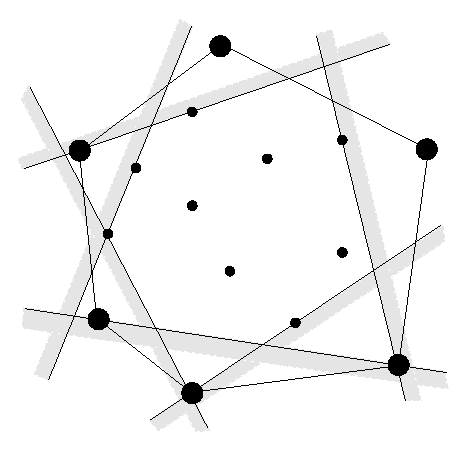
\psfig{file=figs/fig1.eps}
   \caption{\label{fig_1_set}$1$-sets on $S$ and the $1$-zonoid}
 \end{center}
\end{figure}

Now, on the same set $S$, construct all possible $2$-sets. In each
$2$-set, take the mean (represented, in Figure~\ref{fig_2_set}, by the
\textbf{X} on the dotted line segment joining 2 points in each
$2$-set) of the pair of points.  The following lemma shows that by
taking the convex hull of the means from all $2$-sets of $S$, we
obtain the $2$-zonoid of $S$, i.e., $Z_2(S)$ as in Figure
\ref{fig_2_set}.  In a similar fashion, zonoids up to depth $n$ can be
constructed.  Since $Z_n(S)$ is the mean of the points in $S$, it is a
unique point and is the center of gravity of the points in $S$.

\begin{figure}
 \begin{center}
   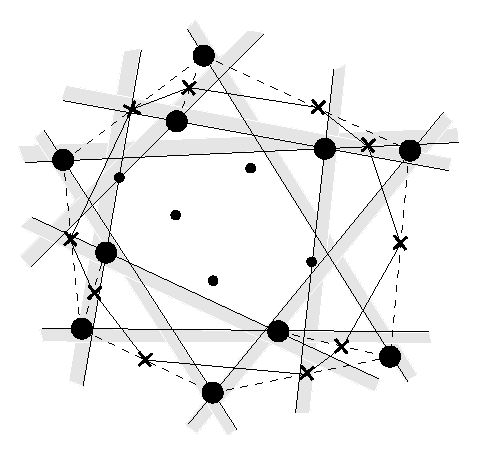
\psfig{file=figs/fig2.eps}
   \caption{\label{fig_2_set}$2$-sets on $S$ and the $2$-zonoid}
 \end{center}
\end{figure}

\begin{lemma}\label{lemma_bijection}
Given a set $S$ of $n$ points in $\mathbb{R}^2$ and an integer $1 \le
k \le n$, there is a bijection between the vertices of $Z_k(S)$ and
the $k$-sets of $S$.
\end{lemma}

\begin{proof}
Consider the mapping $f$ that takes a $k$-set $S'\subseteq S$ onto a
vertex of $Z_k(S)$ using the equation $f(S')=\frac{1}{k}\sum_{p\in S'}
p$.  We will show that $f$ is a bijection between the $k$-sets of $S$ and
the vertices of $Z_k(S)$.

To see that $f$ is one-to-one, consider two $k$-sets $S_1$ and $S_2$.
We need to show that the points $p_1=\frac{1}{k}\sum_{p\in S_1}p$ and
$p_2=\frac{1}{k}\sum_{p\in S_2}p$ are distinct.  The set $S_1$ is the
intersection of $S$ with a halfplane $h$ bounded by a line $\ell$
having inner normal $d$.  The numbers $S_1\cdot d=\{p\cdot d:p\in
S'\}$ are the $k$ largest values in the set $S\cdot d=\{p\cdot
d:p\in S\}$.  It follows
that $p_1\cdot d
> p_2\cdot d$, so $p_1\neq p_2$, as required.

To see that $f$ is onto, we observe that any vertex $v$ of $Z_k(S)$ is
extreme in some direction $d$.  In fact, $v=\frac{1}{k}\sum_{x\in S'}
x$, where $S'$ is a subset of the extreme-most $k$ points of $S$ in
direction $d$.  But then $S'$ is a $k$-set of $S$ since it can be
separated from $S$ by a line $\ell$ perpendicular to $d$.
\end{proof}



\subsection{Review of duality}\label{subsection_review_of_duality}

Let $p = (p_1, p_2)$ denote a point in the plane. The dual of $p$,
denoted by $p^*$, is the line denoted by $p^* = \{(x,y) : y = p_1x -
p_2\}$. The dual of the line $l = \{(x,y) : y = ax + b\}$ is the point
$l^* = (a,-b)$.  
We say that the duality transform maps objects from the \emph{primal}
plane to the \emph{dual} plane. This transform has the following
properties:

\begin{itemize}
\item It is \emph{incidence preserving}: $p \in l$ if and only if $l^*
\in p^*$.

\item It is \emph{order preserving}: $p$ lies above $l$ if and only if $l^*$ lies above $p^*$.
\end{itemize}

A set of lines is said to be in general position if no three of the
lines pass through a common point and two of the lines are parallel.
It follows from the above properties that a set of points in general
position is dual to a set of lines in general position. For a more
detailed explanation of duality see, e.g., Edelsbrunner's book
\cite{edelsbrunner_book}.

\subsection{Correspondence between zonoids and $k$-level}\label{subsection_correspondence_between_zonoids_and_klevel}

The $k$-level of a set $L$ if $n$ lines is defined as the the set of
all points that lie on exactly one line of $L$ and strictly below
$k-1$ lines of $L$. If the lines in $L$ are dual to a set $P$ of
points then each  point $p$ on the $k$-level of $L$ is the dual of a
line $p^*$ that contains one point of $P$ and has exactly $k-1$ points
of $P$ above it.  That is, $p^*$ has a $k$-set of $P$ on or above it.
Similarly, a point on the $(n-k)$-level of $L$ is the dual of a line
with a $k$-set of $P$ on or below it.

\begin{figure}
 \begin{center} 
   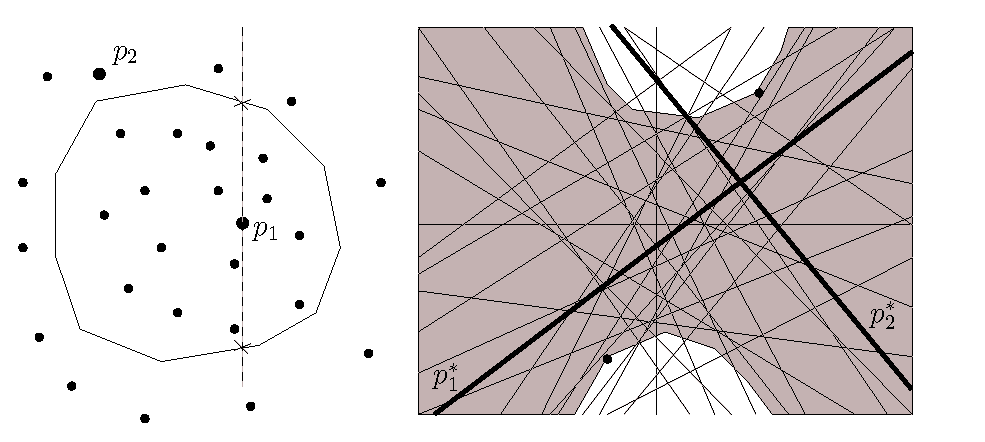
\psfig{file=figs/fig4.eps}
   \caption{A $k$-zonoid in primal and dual}
   \label{fig_primal_dual}
 \end{center}
\end{figure}

We describe the $k$-zonoid in both the primal and the dual settings
and show the relationship between them. The left part of Figure
\ref{fig_primal_dual} represents the primal and the right part, the
dual. The upper (lower) convex hull of points in the primal
corresponds to the upper (lower) envelope of the dual lines in the
dual. In the primal, we construct a $k$-zonoid, for some $k$. In the
dual, this is the shaded region. The upper and lower boundaries of the
shaded region are also convex, because the corresponding boundaries of
the $k$-zonoid in the primal are convex. 

The $k$-zonoid in the primal can be constructed (inefficiently) by
finding all possible $k$-sets, taking the mean of $k$ points in each
$k$-set and taking the convex hull of the resulting point set. In the
dual, this corresponds to constructing the $k$-level (respectively the
$(n-k)$-level) and then, for each vertex that has $k$ lines on and
above it, we draw an upwards (respectively downwards) vertical ray
through it and compute the mean of the $k$ lines that intersect this
vertical ray. These ``mean segments'' are then joined to get the
boundary of the shaded region in Figure \ref{fig_primal_dual}. It may
be observed here that for each vertex on the upper (respectively
lower) boundary of the dual of the $k$-zonoid, there is a vertex
directly below (respectively above) it on the $k$-level (respectively
the $(n-k)$-level). 

Although the number of $k$-sets and the number of vertices of the
$k$-level are different, their sizes are within a constant factor of
each other \cite{edelsbrunner_book}. Dey
\cite{improved_bounds_on_planar_ksets_and_klevels} proves an
$O(nk^{\frac{1}{3}})$ upper bound on the complexity of planar
$k$-levels, which is also an upper bound for the number of planar
$k$-sets. Since we showed that there is a bijection between the
$k$-sets of a point set $S$ and the vertices of $Z_k(S)$ in Lemma
\ref{lemma_bijection}, Dey's result implies an $O(nk^{\frac{1}{3}})$
upper bound on the number of vertices of a $k$-zonoid in
$\mathbb{R}^2$.

Sharir et al.\ \cite{an_improved_bound_for_ksets_in_three_dimensions}
show that the number of $k$-sets in a set of $n$ points in
$\mathbb{R}^3$ is $O(nk^{\frac{3}{2}})$. This implies that, in
$\mathbb{R}^3$ the $k$-zonoid of an $n$ point set has size
$O(nk^{\frac{3}{2}})$.



\section{Algorithms for zonoids in 2 dimensions}
\label{section_algorithms_for_zonoids_in_2_dimensions}

In this section we present algorithms for zonoid depth. The first few
algorithms follow easily from existing results on $k$-sets and
arrangements. The later algorithms are somewhat more involved.

\subsection{Computing a depth contour}
\label{subsection_computing_a_depth_countour}

Chan \cite{remarks_on_klevel_algorithms_in_the_plane} describes an
algorithm for computing the $k$-level in a set of $n$ lines that runs
in $O(n \log n + nk^{\frac{1}{3}})$ expected time. Using this
algorithm, the $k$-level and the $(n-k)$-level can be constructed in
$O(n \log n + nk^{\frac{1}{3}})$ expected time. This algorithm is
easily augmented to output the $k$-zonoid. 

\begin{theorem}\label{theorem_build_k_zonoid}
Given a set $S$ of $n$ points in $\mathbb{R}^2$ and an integer $1 \le
k \le n$, the $k$-zonoid $Z_k(S)$ can be computed in $O(n \log n +
nk^{\frac{1}{3}})$ expected time.
\end{theorem}


\subsection{Computing a depth map}\label{subsection_computing_a_depth_map}

Applying Theorem \ref{theorem_build_k_zonoid} $n$ times for $k$ from 1
to $n$ gives us an algorithm to compute a depth map in $O(n^2 \log n +
n^2 k^{\frac{1}{3}})$ expected time. But the relationship between
$k$-zonoids, $k$-levels and $(n-k)$-levels allows us to compute
$Z_1(S),\ldots,Z_n(S)$ in $O(n^2)$ time by computing the arrangement
of the dual lines \cite{edelsbrunner_book}.

\begin{theorem}\label{theorem_build_1_to_n_zonoids}
Given a set $S$ of $n$ points in $\mathbb{R}^2$,
$Z_1(S),\ldots,Z_n(S)$ (i.e. the depth map) can be computed in
$O(n^2)$ time.
\end{theorem}

Once we have computed the $Z_1(S),\ldots,Z_n(S)$, we can preprocess
them for point location using Kirkpatrick's planar point location
algorithm \cite{optimal_search_in_planar_subdivisions} so that we can
determine the zonoid depth of any point in $O(\log n)$ time. 

\begin{theorem}\label{theorem_point_location}
Given a set $S$ of $n$ points in $\mathbb{R}^2$,
after preprocessing requiring $O(n^2)$ time and space the zonoid
depth of any query point $p$ can be computed in $O(\log n)$ time.
\end{theorem}

\subsection{Testing if a zonoid contains a point}
\label{subsection_testing_if_a_zonoid_contains_a_point}

In this section, we study the following decision problem: Given a set
$S$ of $n$ points in general position, a query point $p$ and an
integer $1 \le k \le n$, determine whether $p$ is contained in
$Z_k(S)$. 

Consider again Figure \ref{fig_primal_dual}. In the primal, if the
point $p_1$ were to be moved upwards along a vertical line passing
through $p_1$, then the line $p_1^*$ also moves upwards in the dual,
parallel to itself. When $p_1$ hits the $k$-zonoid boundary, $p_1^*$
becomes tangent to the boundary of the dual of the $k$-zonoid. This
leads to the following idea: In the primal, first determine the
vertices of the zonoid with smallest and largest $x$-coordinate.  If
the point $p_1$ is not in the vertical strip between these two points
then $p_1$ is not the in the zonoid.

Otherwise, draw a vertical line through the point $p_1$. This line
intersects the boundary of the $k$-zonoid in 2 points.  Finding these
intersection points is equivalent to finding the points at which the
vertical translation of line $p_1^*$ becomes tangent to the boundaries
of the dual of the $k$-zonoid. Once they are found, it can be easily
said whether $p_1$ is inside or outside the $k$-zonoid by comparing
the $y$-coordinates of the intersection points with that of  $p_1$.
Hereafter, we concentrate on finding that vertex on the upper boundary
of the dual of the $k$-zonoid at which $p_1^*$ is tangent. Such a
vertex on the lower boundary can be found in a symmetric manner. 

The algorithm that we use is inspired by the planar ham-sandwich
algorithm of Lo et al.\ \cite{algorithms_for_ham_sandwich_cuts}. In
their algorithm, Lo et al.\ are searching for a particular vertex on
the median level of the arrangement of lines in the dual. In the
primal, this vertex corresponds to a line passing through 2 points and
bisecting this set. In our problem, we are searching for a particular
vertex on the $k$-level that defines the point on the upper boundary
of the dual of the $k$-zonoid at which a vertical translation of
$p_1^*$ is tangent.

In the following, we describe and analyze our algorithm in detail even
though the algorithm and its analysis are more or less the same as the
algorithm of Lo et al.  This is because we will be modifying this
algorithm in
Section~\ref{subsection_computing_the_zonoid_depth_of_a_point} to
solve the same problem for weighted points.  Describing and analyzing
the modified algorithm requires an understanding of the original
algorithm and its analysis.

\begin{figure}
 \begin{center} 
   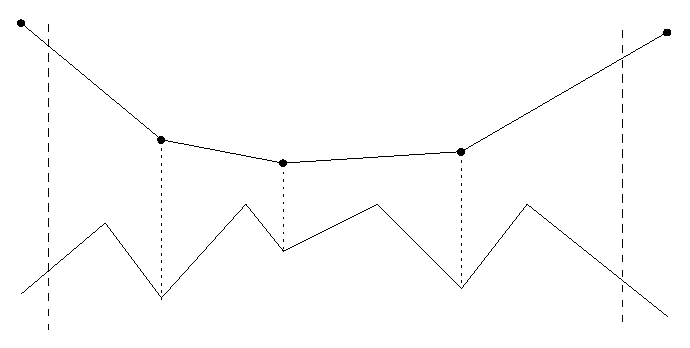
\psfig{file=figs/fig5.eps}
   \caption{\label{fig_vertical_strip}Vertical strip $V$ showing the $k$-level and corresponding upper boundary of the dual of the $k$-zonoid}
 \end{center}
\end{figure}

\begin{figure}
 \begin{center}
   \begin{center}\begin{tabular}{ccc} 
   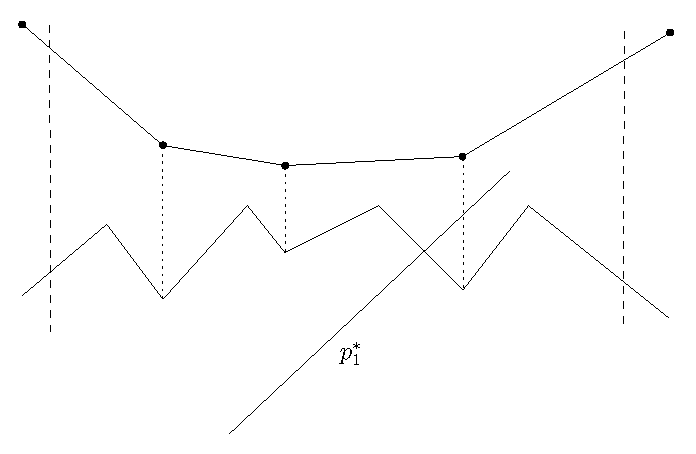
\includegraphics[width=1.8in]{figs/fig5a} &
   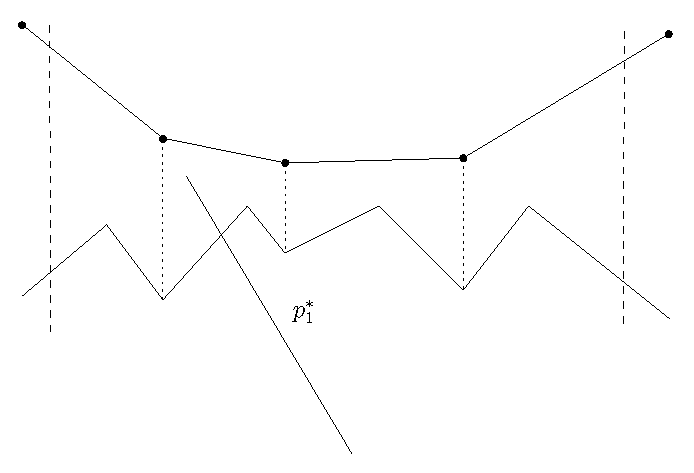
\includegraphics[width=1.8in]{figs/fig5b} &
   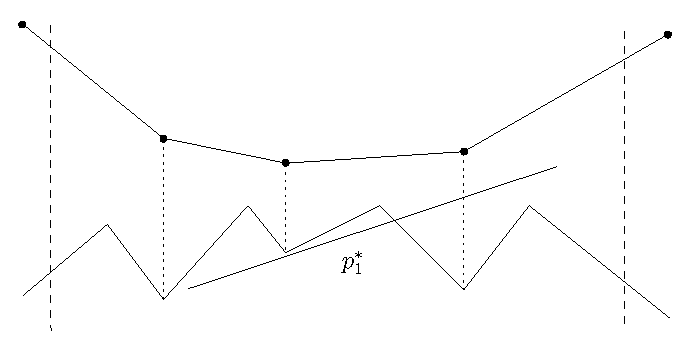
\includegraphics[width=1.8in]{figs/fig5c} \\
   (a) & (b) & (c)
   \end{tabular}\end{center}
   \caption{\label{fig_vertical_strip_abc} The vertical translation of $p_1^*$ is tangent to the
upper boundary of the dual of the $k$-zonoid to (a)~the \emph{right}
of $V$, (b)~the left of $V$ and (c)~inside of $V$.}
 \end{center}
\end{figure}


Consider an open vertical strip $V$ in the dual, as in Figure
\ref{fig_vertical_strip}, showing the $k$-level and the corresponding
convex upper boundary of the dual of the $k$-zonoid.  Our algorithm
requires a method to determine whether a vertical translation of $p_1^*$
becomes tangent to the upper boundary of the dual $k$-zonoid  (1)~to
the left of the strip $V$, (2)~in
the strip $V$, or (3)~to the right of
the strip $V$.  To determine this, we compute the slope $s_\ell$ of
the dual $k$-zonoid edge that intersects the left boundary of $V$ and
the slope $s_r$ of the dual $k$-zonoid edge edge that intersects the
right boundary of $V$.  Both these computations can be done in $O(n)$
time using an $O(n)$ time selection algorithm to select the
intersection of the $k$-level with each of these two vertical lines
bounding $V$.  If $s$ is
the slope of $p^*$ then either
\begin{enumerate}
\item $s \le s_\ell < s_r$ in which case a vertical translation of
$p_1^*$ is tangent to the dual $k$-zonoid at some point to the left of
$V$, 
\item $s_\ell < s < s_r$ in which case a vertical translation of
$p_1^*$ is tangent to the dual $k$-zonoid at some point in 
$V$, or
\item $s_\ell < s_r \le s$ in which case a vertical translation of
$p_1^*$ is tangent to the dual $k$-zonoid at some point to the right
of $V$.
\end{enumerate}

The above method is used in conjunction with the following lemma
(that appears in Ref.~\cite{algorithms_for_ham_sandwich_cuts}) for
subdividing an arrangement into vertical strips:

\begin{thma}
Let $L$ be a set of $n$ lines in the plane in general position, let
$\alpha < 1$ be a prescribed positive constant and let $V$ be a
vertical strip. In $O(n)$ time, $V$ can be partitioned into vertical
strips $V_1, V_2, \ldots, V_C$ (where $C = C(\alpha)\le 2/\alpha$ is a function
that depends only on $\alpha$), such that each $V_i$ contains at most
$\alpha N$ of the $N = {n \choose 2}$ vertices of arrangement of
$L$. 
\end{thma}

In our problem, we apply the Subdivision Lemma in the dual. Let our
strip $V=\mathbb{R}^2$.  We want to subdivide $V$ into substrips so
that each substrip contains at most ${n\choose 2}/20$ of the
total number of intersections in $V$. The reason for this choice will
become clear shortly. So we set $\alpha = {1}/{20}$ and get at
most $C(1/20)\le 40$ strips $V_1, V_2, \ldots, V_{40}$.

We now have 40 open vertical strips and we can determine in $O(n)$
time, using the method described above, a strip that $V_i$ contains
the upper boundary vertex at which a line parallel to $p_1^*$ is
tangent. 

\begin{figure}
 \begin{center}
   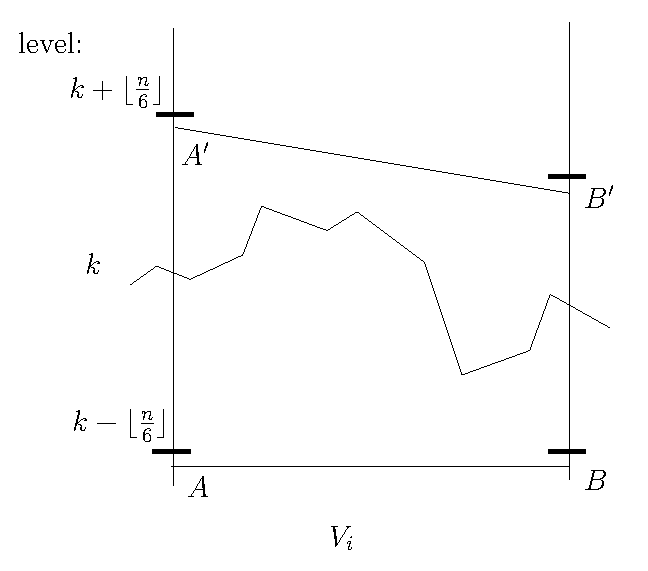
\psfig{file=figs/fig6.eps}
   \caption{\label{fig_trapezoid}Figure showing how we build the trapezoid $ABB^{\prime}A^{\prime}$}
 \end{center}
\end{figure}

In $V_i$, we build a trapezoid $T = ABB^{\prime}A^{\prime}$, as shown
in Figure \ref{fig_trapezoid}. The points $A$ on the left vertical
line and $B$ on the right vertical line lie just below the $k -
\lfloor\frac{n}{6}\rfloor$ level of the lines in the dual and the
points $A^{\prime}$ and $B^{\prime}$ lie just below the $k +
\lfloor\frac{n}{6}\rfloor$ level of the lines in the dual (if $k -
\lfloor\frac{n}{6}\rfloor \le 0$, then $A$ and $B$ are chosen below
all lines, and similarly for the top side).

\begin{lemma}\label{lemma_trapezoid}
The top and bottom sides of the trapezoid $T$ intersects at most 
$n/3$ dual lines each.
\end{lemma}

\begin{proof}
Let $u$ be the number of lines intersecting the side $AB$ of $T$
\emph{upwards}, i.e., these lines have $A$ above and $B$ below them.
Let $d$ be the number of lines intersecting $AB$ of $T$
\emph{downwards}. Since $A$ and $B$ are each on the
$k-\lfloor\frac{n}{6}\rfloor$ level, we have $u = d$. But every
\emph{upwards} line intersects every \emph{downwards} line in the
strip $V_i$, hence $V_i$ contains at least $ud=u^2$ intersections.

Each
strip $V_i$ was created so that it has at most
$\frac{1}{20}{n\choose 2}$ intersections. Therefore, 
            $u^2 \le {n \choose 2}/20$, which implies that
$u \le n/\sqrt{40} \le n/6$.
Thus, $u+d\le n/3$ is the number of lines intersecting side $AB$ of
trapezoid $T$. A symmetric argument shows that the number of lines
intersecting 
$A^{\prime}B^{\prime}$ is also at most $n/3$.
\end{proof}

The 2 vertical sides of the trapezoid $T$ are also intersected by at
most $\frac{n}{3}$ lines each, because of our choice of the levels of
the points $A, B, B^{\prime}$ and $A^{\prime}$. So each side of $T$ is
intersected by $\le \frac{n}{3}$ lines, hence we have at most
$\frac{4n}{3}$ intersections altogether. Each line that intersects the
trapezoid contributes 2 to this sum, so we have at most $\frac{2n}{3}$
lines that intersect the trapezoid, which means $\frac{n}{3}$ lines
pass outside the trapezoid.

\begin{lemma}\label{lemma_trapezoid_containment}
Within the vertical strip $V$, the $k$-level is completely contained
in $T$. 
\end{lemma}

\begin{proof}
Suppose that the $k$-level goes below the bottom side $AB$ of $T$. Then
some point $C$ on this side has level greater than $k$. Since both
$A$ and $B$ have level $k - \lfloor\frac{n}{6}\rfloor$, each of the
segments $AC$ and $BC$ have to be intersected by more than
$\frac{n}{6}$ lines. But this contradicts Lemma \ref{lemma_trapezoid}.
Similarly, the $k$-level can not be above the top side $A'B'$ of $T$
and must therefore be contained in $T$.
\end{proof}

Based on Lemmata \ref{lemma_trapezoid} and
\ref{lemma_trapezoid_containment}, the $\frac{n}{3}$ lines that pass
outside trapezoid $T$ can be safely discarded since the intersection
of the $k$-level with the strip $V_i$ is completely contained in $T$.
However, when we discard the lines that lie above $T$, we remember
their mean, since this will be needed to compute slopes in recursive
calls to the algorithm.

\comment{
It may be observed that until recently in our discussion, we were trying to find the vertex on the boundary of the dual of the $k$-zonoid at which line $p_1^*$ becomes a tangent. But above we show that it is the $k$-level that lies completely inside the trapezoid $T$ and the vertex point is being searched for on the $k$-level, not on the boundary of the dual of the $k$-zonoid. This is because, 
\begin{enumerate}
\item we do not explicitly construct the $k$-zonoid in the dual,
\item each vertex on the boundary of the dual of the $k$-zonoid is calculated by taking the mean of the $k$ lines above a $k$-level vertex,
\item even though we disregard lines above and passing outside the trapezoid $T$, their equations can be associated with each $k$-level vertex and the corresponding $k$-zonoid dual vertex be computed, as need arises.  
\end{enumerate}
}

After we build the trapezoid $T$ and discard $\frac{n}{3}$ of the
lines passing outside $T$, we reconstruct open vertical strips inside
this trapezoid for the remaining $\frac{2n}{3}$ lines and get a new
trapezoid and search within it. Thus, each iteration (or recursive
invocation) runs in time linear in the number of lines and discards a
constant fraction of the lines. Hence the algorithm runs in $O(n)$
time. This yields the following theorem.

\begin{theorem}\label{theorem_decision_problem}
Given a set $S$ of $n$ points in $\mathbb{R}^2$, a query point $p$ and
an integer $1 \le k \le n$, we can determine in $O(n)$ time whether or not $p$ lies inside or outside the $k$-zonoid $Z_k(S)$. More generally, we can compute the intersection of $Z_k(S)$ with any line in $O(n)$ time.
\end{theorem}

\subsection{Computing the zonoid depth of a point}
\label{subsection_computing_the_zonoid_depth_of_a_point}

Theorem~\ref{theorem_decision_problem} offers a means of solving the
\emph{decision problem}: Is $p\in Z_k(S)$?  In this section we solve
the optimization problem:  What is the zonoid depth of $p$? I.e., the
what is the maximum value $k$ such that $p\in Z_k(S)$.  To do this, we
use a general technique due to Chan
\cite{geometric_applications_of_a_randomized_optimization_technique}
for converting decision algorithms into optimization algorithms.  Let
$\depth(p,S)$ denote the zonoid depth of $p$ with respect to $S$.
Roughly stated, Chan's algorithm requires
\begin{enumerate}

\item (Decision Algorithm) a decision algorithm to decide whether
$\depth(p,S)$ is at least $k$ and

\item (Decomposition into Subproblems) an algorithm to express
$\depth(p,S)$ as $\max\{\depth(p,S_i):1\le i\le r\}$ where $r$ is a
constant and each $|S_i|\le \alpha|S|$ for some constant $\alpha < 1$.
\end{enumerate}

If these conditions are met, then Chan's technique
allows us to solve the optimization problem
efficiently.\footnote{There is a more precise statement of Chan's very
powerful optimization technique, but our application of the technique
does not fit the usual requirements of this statement, so we omit it
here.  The interested reader is referred to Chan's original paper
\cite{geometric_applications_of_a_randomized_optimization_technique}}
Initially, it seems that Theorem~\ref{theorem_decision_problem}
satisfies Requirement~1 above.  However, to satisfy Requirement~2 we
need to define a slightly more general problem on weighted zonoids.
This, in turn, means that we need a slightly more general algorithm to
satisfy Requirement~1.


\subsubsection{Weighted Zonoids}
\label{section_decision}

Let $S = \{p_1, p_2, \ldots, p_m\}$ be a set of $m$ points in general
position and let each point $p_i$ have an associated positive integer
weight $w(p_i)=w_i$.  Let $n=\sum_{i=1}^m w_i$.  The \emph{$w$-weighted
$k$-zonoid of $S$} is defined as

\[ Z_k(S,w) = \left\{\sum_{i=1}^{m}\lambda_iw_ip_i \mid 0 \le \lambda_i \le \frac{1}{k},\, \sum_{i=1}^{n} \lambda_i = 1 \right\} \]

Note that the original definition of zonoid depth is a special case of
this definition in which $n=m$ and $w_i=1$ for all $1\le i\le m$.
Also observe that, since the $w_i$ are positive integers, any problem
on weighted zonoids can be converted into an equivalent unweighted
zonoid problem by simply replacing each point $p_i$ by $w_i$
infinitesmally close points. Thus, for example,
Theorem~\ref{theorem_decision_problem} could be applied to compute the
intersection of any line with a weighted zonoid in $O(n)$ time.
However, this observation is insufficient for our purposes, and we
need an algorithm whose running time depends more on the number of
points $m$ than the total weight $n$ of those points.

\begin{lemma}
Let $S$, $n$, $w$ and $m$ be defined as above.  Then, the intersection
of any line with $Z_k(S,w)$ can be computed in $O(m\log (n/m) + m)$
time.
\end{lemma}

\begin{proof} We apply a slight modification of the algorithm given by
Theorem~\ref{theorem_decision_problem}.  In this modification, the
algorithm works on the \emph{weighted $k$-level}.  (The weight of a
point $p$ is the sum of the weights of all lines that pass through or
above $p$. The weighted $k$-level is the lower envelope of all points
having weight at least $k$.)  The modified algorithm is almost
identical to the previous algorithm except that, where the previous
algorithm uses a linear-time selection algorithm to compute the
intersection of the $k$-level with a vertical line, the modified
algorithm makes use of a linear-time weighted selection algorithm.
Also, where the previous algorithm uses the Subdivision Lemma, the
modified algorithm uses a weighted Subdivision Lemma which guarantees
that each open strip contains at most ${n\choose 2}/20$ \emph{weighted
intersections}.  (The weight of an intersection between line $p_i^*$
and $p_j^*$ is $w_i\times w_j$.) Otherwise, the algorithm is identical
to the previous algorithm.  At each round, the algorithm runs in
$O(m)$ time, where $m$ is the number of lines at the beginning of the
round and reduces the total weight $n$ of those lines (but not
necessarily the number of lines $m$) by a factor of $2/3$.
Correctness of the algorithm follows from exactly the same argument as
the original algorithm.

To analyze the running time of the modified algorithm we observe that the
$i$th iteration of the algorithm takes $O(m_i)$ time, where $m_i$ is
the number of lines at the beginning of the $i$th iteration.
Furthermore, $m_i\le n_i$, where $n_i$ is the total weight of those
lines. Finally, the value of $n_i$ decreases by a factor of $2/3$
during every iteration. These observations imply that the overall
running time of the algorithm is bounded by 
\begin{eqnarray*} 
  T_{n,m}
    & \le & \sum_{i=0}^{\infty} O(m_i) \\ 
    &\le& \sum_{i=0}^{\infty} O(\min\{(2/3)^in, m\})  \\ 
    & = & O(m\log (n/m)) + O(m) \enspace ,
\end{eqnarray*} 
as required.  
\end{proof}

\subsubsection{The Decomposition into
Subproblems}\label{section_decomp}

The algorithm for weighted zonoids from the previous section will play
the role of the decision algorithm in our application of Chan's
optimization technique.  In this section, we describe the
decomposition into subproblems required to apply Chan's technique.

Assume $S$, $w$ and $p$ are the inputs to our problem.  That is, we
want to compute the $w$-weighted zonoid depth of $p$ with respect to
$S$.   We can decompose this problem into 4 subproblems $S_1$, $S_2$,
$S_3$, and $S_4$ as follows: In $O(m)$ time, we select two lines that partition the
set $S$ into 4 quadrants $Q_1$, $Q_2$, $Q_3$, and $Q_4$ that
each contain roughly $m/4$ points, using Megiddo's 
algorithm \cite{partitioning_with_two_lines_in_the_plane}. Subproblem
$S_1$ contains 3 consecutive quadrants, say $Q_1, Q_2, Q_3$, and a
single point which is the weighted average of all the points in
$Q_4$ and whose weight is the sum of the weights of all points in
$Q_4$.  That is we create a new point $p_\ell$ with, 
\[
     w_\ell = \sum_{p_i\in Q_4} w_i
\]
and
\[
     p_\ell = \frac{1}{w_\ell}\sum_{p_i\in Q_4} w_ip_i \enspace .
\]
Thus, $S_1$ contains $\frac{3m}{4}+1$ points. We define the sets
$S_2$, $S_3$, and $S_4$ in a similar manner.  We define $depth(p,S_i)$
as the weighted zonoid depth of point $p$ in problem $S_i$. It follows
immediately from the definition of weighted zonoids that 
this decomposition produces strictly smaller zonoids, i.e.
$Z_k(S_i,w) \subseteq Z_k(S,w)$ and does not change the center, i.e.,
$Z_n(S_i)=Z_n(S)$.  The following lemma shows that this
decomposition satisfies the second requirement of Chan's optimization
technique.

\begin{lemma}\label{lemma_final} Let $S$ and $S_1$, $S_2$, $S_3$, and
$S_4$ be defined as above.  Then
\begin{itemize} \item[a.]
$depth(p,S_i) \le depth(p,S)$ for each $1 \le i \le 4$, \item[b.]
$depth(p,S) = \max\{depth(p,S_i) \mid 1 \le i \le 4\}$ \end{itemize}
\end{lemma}

\begin{figure}
 \begin{center}
   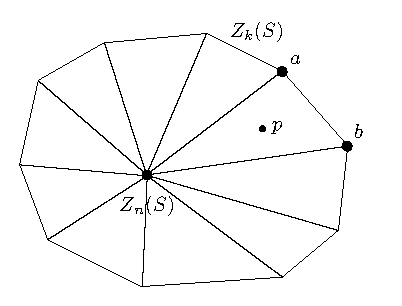
\psfig{file=figs/fig7.eps, width=3in, height=2.5in}
   \caption{\label{fig_for_proof}Partitioning the $Z_k(S)$ zonoid into triangles}
 \end{center}
\end{figure}

\begin{proof} Part \textit{a} follows from the observation that
$Z_k(S_i) \subseteq Z_k(S)$. To see why Part \textit{b} is true,
suppose $depth(p,S) = k$ and partition $Z_k(S)$ into triangles by
drawing segments joining $Z_n(S)$ to each of the vertices of $Z_k(S)$,
as shown in Figure \ref{fig_for_proof}. The point $p$ lies in one of
these triangles, say with vertices $Z_n(S), a \hspace{1mm} \mbox{and}
\hspace{1mm} b$. The points $a$ and $b$ correspond to two $k$-sets
that have $k-1$ points in common. Indeed, there are two
infinitesimally close lines $l_a$ and $l_b$ such that $l_a$ defines
the $k$-set for $a$ and $l_b$ defines the $k$-set for $b$. Since $l_a$
and $l_b$ are infinitesimally close, they intersect at most three of
the open quadrants $Q_1, \ldots, Q_4$. Wlog suppose they miss $Q_4$. Then
it is not hard to see that $Z_k(S_1,w)$ has $a$ and $b$ as vertices.
Furthermore, $Z_k(S_1)$ contains $Z_n(S)$ and is convex, so it
contains $p$. Therefore $depth(p,S_1) \ge k = depth(p,S)$ as required.
\end{proof}

\subsubsection{Analysis of Chan's Technique}

Next, we analyze the cost of applying Chan's optimization technique
with the decision algorithm from Section~\ref{section_decision} and
the decomposition algorithm from Section~\ref{section_decomp}.  This
is not quite a standard application of Chan's technique because the
running time of our decision algorithm is a function of both $n$ and
$m$, and our decomposition algorithm only decreases the value of $m$
(and not the value of $n$) in each subproblem. 

If we redo Chan's analysis, we find that the expected number of
decision problems we solve at the $i$th level of recursion is $r^i$
and these decision problems each have total weight $n$ distributed
among $m_i=\alpha^i n$ points.  Here, $r=\ell\ln4+1$,
$\alpha=(3/4)^\ell$ and $\ell$ is an integer parameter that is under
our control.  Therefore, the total expected cost of the algorithm is
bounded by the summation
\[
   T_n = \sum_{i=1}^\infty O\left(r^im_i\log (n/m_i)\right)
   = n\sum_{i=1}^\infty O\left(r^i\alpha^i \log(1/\alpha^i)\right)
   = n\sum_{i=1}^\infty O\left(r^i\alpha^i i\right) \enspace ,
\]
which solves to $O(n)$ provided that $r\alpha < 1$.  The condition
$r\alpha < 1$ is easily ensured by choosing a sufficiently large
value of $\ell$.  This completes the proof of our final theorem:

\begin{theorem}\label{theorem_final}
Given a set $S$ of $n$ points in $\mathbb{R}^2$ and a query point $p$,
we can find the largest integer $k$ for which $p$ lies inside $Z_k(S)$
(i.e., the zonoid depth of $p$) in $O(n)$ expected time. 
\end{theorem}

\section{Conclusions and open problems}\label{section_conclusions_and_open_problems}

We have given algorithms for solving several computational problems
related to zonoid depth for 2-dimensional (bivariate) data.
In particular,  we have given 

\begin{enumerate}
\item an $O(n\log n+nk^{\frac{1}{3}})$ algorithm to compute $Z_k(S)$, i.e. the zonoid depth contour of depth $k$,	
\item an $O(n^2)$ algorithm to compute $Z_1(S),\ldots,Z_n(S)$, i.e. the zonoid depth map,
\item a linear time algorithm to test whether a zonoid $Z_k(S)$ contains a point, and
\item a linear time algorithm to compute the zonoid depth of a point.
\end{enumerate}
Results 2, 3 and 4 are optimal. An improvement on Algorithm 1 would require a breakthrough on the (30 year old) planar $k$-set problem. 

This article only deals with zonoid depth problems in 2 dimensions
and, besides the work by Dyckerhoff et al.\
\cite{zonoid_data_depth_theory_and_computation} and Bern and Eppstein
\cite{bern-eppstein-01}, no work has been done regarding zonoid depth
problems in dimensions 3 and higher.  In particular, for small
(constant)
dimensions it is a challenge to find algorithms for computing zonoid
depth that do not rely on linear programming in high (a function of
$n$) dimensions.

\bibliographystyle{plain}
\bibliography{refs}

\end{document}
